\documentclass[10pt]{article} % FORMAT CHANGE
\usepackage[dvips]{graphicx}  %hm, does this include epsfig? i guess so 
\usepackage{times}

\graphicspath{{./}{figs/}} 

\pagestyle{plain}

\addtolength{\hoffset}{-2cm}
\addtolength{\textwidth}{4cm}

\addtolength{\voffset}{-1.5cm}
\addtolength{\textheight}{3cm}

\setlength{\parindent}{0pt}
\setlength{\parskip}{12pt}


\title{PVFS 2 Concepts: The new guy's guide to PVFS}

\author{PVFS Development Team}

\begin{document}
\maketitle

\begin{verbatim}$Id: concepts.tex,v 1.3 2006-09-13 20:22:43 vilayann Exp $\end{verbatim}
\section{Introduction}

PVFS2 represents a complete redesign and reimplementation of the
parallel file system concepts in PVFS1.  PVFS2 has new entities acting
in new ways on new objects.  This document will serve as an introduction
to the terminology and concepts used in the other pvfs2 documents.

% i really don't know what sections everything will end up in...

\section{Words}
% metaserver, io server,  scheduler, server request
\begin{description}
\item[\em system interface] low-level interface to PVFS.  sits on top of
    the servers.  provides underlying foundation to higher-level
    interfaces like the PVFS library ( libpvfs2 ) and the PVFS VFS
    interface. 
\item[\em distributions] (also ``file distributions'', ``physical
    distribution'' ) set
    of methods describing a mapping from a logical sequence of bytes to
    a physical layout of bytes on PVFS servers.  PVFS1 had one type of
    distribution --  regularly striding data.  PVFS2 will understand
    many distributions, including but not limited to strided, block and
    cyclic. 

% how has the job concept changed since January's rethinking?
\item[\em job ] a PVFS operation requires several steps, called ``jobs''
\begin{description}
  \item[\em job interface] keeps track of progress as an operation
   makes its way through the pvfs2 layers
  \item[\em job structure] 
\end{description}

\item[\em BMI (Buffered Message Interface)] abstracts network communication.  
   Currently BMI supports
   TCP, Myricom/GM, and InfiniBand using either VAPI or OpenIB APIs.
   It has been extended to at least two other protocols not included in the
   distribution.
   
\item[\em flows] a flow describes the movement of file data from client
   initialization to putting bits on disk.  It encompasses both
   transporting data over the network as well as interacting with
   storage devices. ( XXX: scheduler?).  Users tell flow {\em what} they
   want done, and flow figures out {\em how} to accomplish the request.
   Flows are not involved in metadata operations.
   \begin{description}
   \item[\em flow interface] the API for setting up flows
   \item[\em flow protocol] Implements whatever underlying protocol is
   needed for two endpoints to communicate
   \item[\em flow endpoint] the source or destination of a flow 
   \item[\em flow descriptor] data structure representing a flow
   \end{description}
   
\item[\em trove ] stores both keyword-value pairs and data (?)
\begin{description}
  \item{\em storage interface (obsolete)} now called {\em trove}
\end{description}

\item[\em system level objects ] data files, metadata files,
  directories, symlinks
  \begin{description}
    \item[\em metadata] data about data. in the UNIX sense, such things as
      owner, group, permissions, timestamps, sizes.  in the PVFS sense,
      also distribution information.
    \item[\em data] actual contents of file
    \item[\em metafile] contains the metadata for a single PVFS file
    \item[\em datafile] contains some portion of the data for a single PVFS
        file
  \end{description}
% did not define symlinks or directories, as these are not substantially
% different from their unix counterparts.
\item[\em dataspace] logical collections of data 
	\begin{description}
	\item[\em bytestream] arbitrary binary data.  Data is accessed
	with sizes from offsets.
	\item[\em keyval ] a keyword/value pair. Data is accessed by
	resolving a key.
	\end{description}
\item[\em collections ]
\item[\em server request protocol]
\item[\em vtags ] provides a version number for any region of a byte stream 
    or any individual key/value pair.  By comparing the vtag before and
    after an operation, one can ensure consistency.  
\item[\em handle] a 64-bit tag to uniquely identify PVFS objects.
  Re-using handles brings up some ``interesting'' cases.   (aside: what
  if we made the handles 128 bits )
% is instance tag still around?
\item[\em instance tag] in some cases, a handle might refer to two
  distinct files with the same name.  The {\tt instance tag} serves as
  an extra identifier to help ensure consistency
\item[\em pinode] A mechanism for associating information with a handle.  
  Like a linux inode, a {\tt pinode} contains information used by PVFS2
  internally.  

\item[\em gossip ] A logging library.  Internal to clemson?  freshmeat
doesn't have an entry for it, and searching for ``gossip logging
library'' in google turns up a ton of irrelevant searches.
\end{description}

\section{The view from 10,000 feet}

Refer to figure \ref{fig:interface-model} for an idea of how the words above
fit together.

All end-user access to PVFS will still be provided by one of several
front ends (VFS kernel interface, ROMIO, libpvfs) ( {\it what's the
right term here?  API, FE, interface?}).  The new pvfs library has not
been written yet, but there is a good chance it will be largely similar
to the current pvfs library.  The ROMIO and VFS interfaces should remain
largely unchanged to the end user, aside from extensions to take
advantage of new PVFS2 features.

The end-user interfaces converge at the system interface.  If a user
request requires talking to several servers, the system interface
submits a job request for each server to the job manager ( {\it i
presume, if the job mgr can't split up requests that the submission of
multiple jobs happens in the sys-int.  or will the client find out who
he has to talk to after opening the file?}).  Requests for
large or noncontiguous data chunks only need one job as explained below.

The job manager is a fairly thin layer between the system interface and
BMI, trove, and flow.  It should be noted that nearly every request
requires multiple steps ( communicate over the network, read bytes from
storage ...), and each step becomes a job. The job manager provides a
common handle space (terminology?) and thread management to keep
everything progressing.

If the user performs a data operation, the system interface will submit
a flow job.  The system interface knows what {\em has} to happen -- some
bytes from here have to go over there.  The flow job figures out {\em how}
to accomplish the request.  The flow can compute how much data comes from
which servers based on the I/O request and the distribution parameters.
The flow then is responsible for making the right BMI calls to keep the
i/o request progressing. 

Metadata requests go directly to BMI jobs.  ... ({\em client requests
will never go directly to trove, right? })

Wind back up the protocol stack to the servers for a moment.  We'll
come back to BMI in a bit.   From the client side, all jobs are
``expected'': the client asks for something to happen and can test for
completion of that job.  PVFS2 servers can additionally receive
``unexpected'' jobs, generally (always?) when a client initiates a
request from a server.  ({\em where can i find more information about
the ``request handler'' and the ``op state machine'' in
figure \ref{fig:interface-model} ?} ) 

The job manager works the same way for the server as it does for the
client, keeping track of BMI, trove, and flow jobs.  

Figure \ref{fig:setmeta-protocol} shows a setmeta operation.  The client
starts a BMI job to send a request to the meta server.  The server then
receives a job indicating that an unexpected BMI message has arrived.
The server then issues a Trove job to store the metadata, and issues a
BMI Job to send an ack.  The client does a BMI job to receive the ack. 
A setmeta requires 2 jobs on the client side (send request, receive          
ack), and 3 jobs on the server side (receive request, do meta operation,        
send ack).  {\em (hrm? so ``unexpected'' isn't completely true? the
server expects a request enough to post a receive )}

Data operations are largely similar to metadata operations:
the client posts jobs to send the request and receive the response, the
server posts jobs to receive the request, do the operation, and send an
ack.  The difference is that a flow does the work of moving data. ( XXX:
i have a figure for this.  is this type of figure useful? )

Jobs and flows use BMI abstractions anytime they have to communicate
over the network.  The BMI level resolves these abstract "connections"
into real network activity.  BMI will either open a TCP socket, do some
GM magic, or do whatever the underlying system network needs done to
move bytes. 

Similarly, jobs and flows use trove abstractions and let trove deal with
the actual storage of bytestream and keyval objects


\begin{figure}
\centering
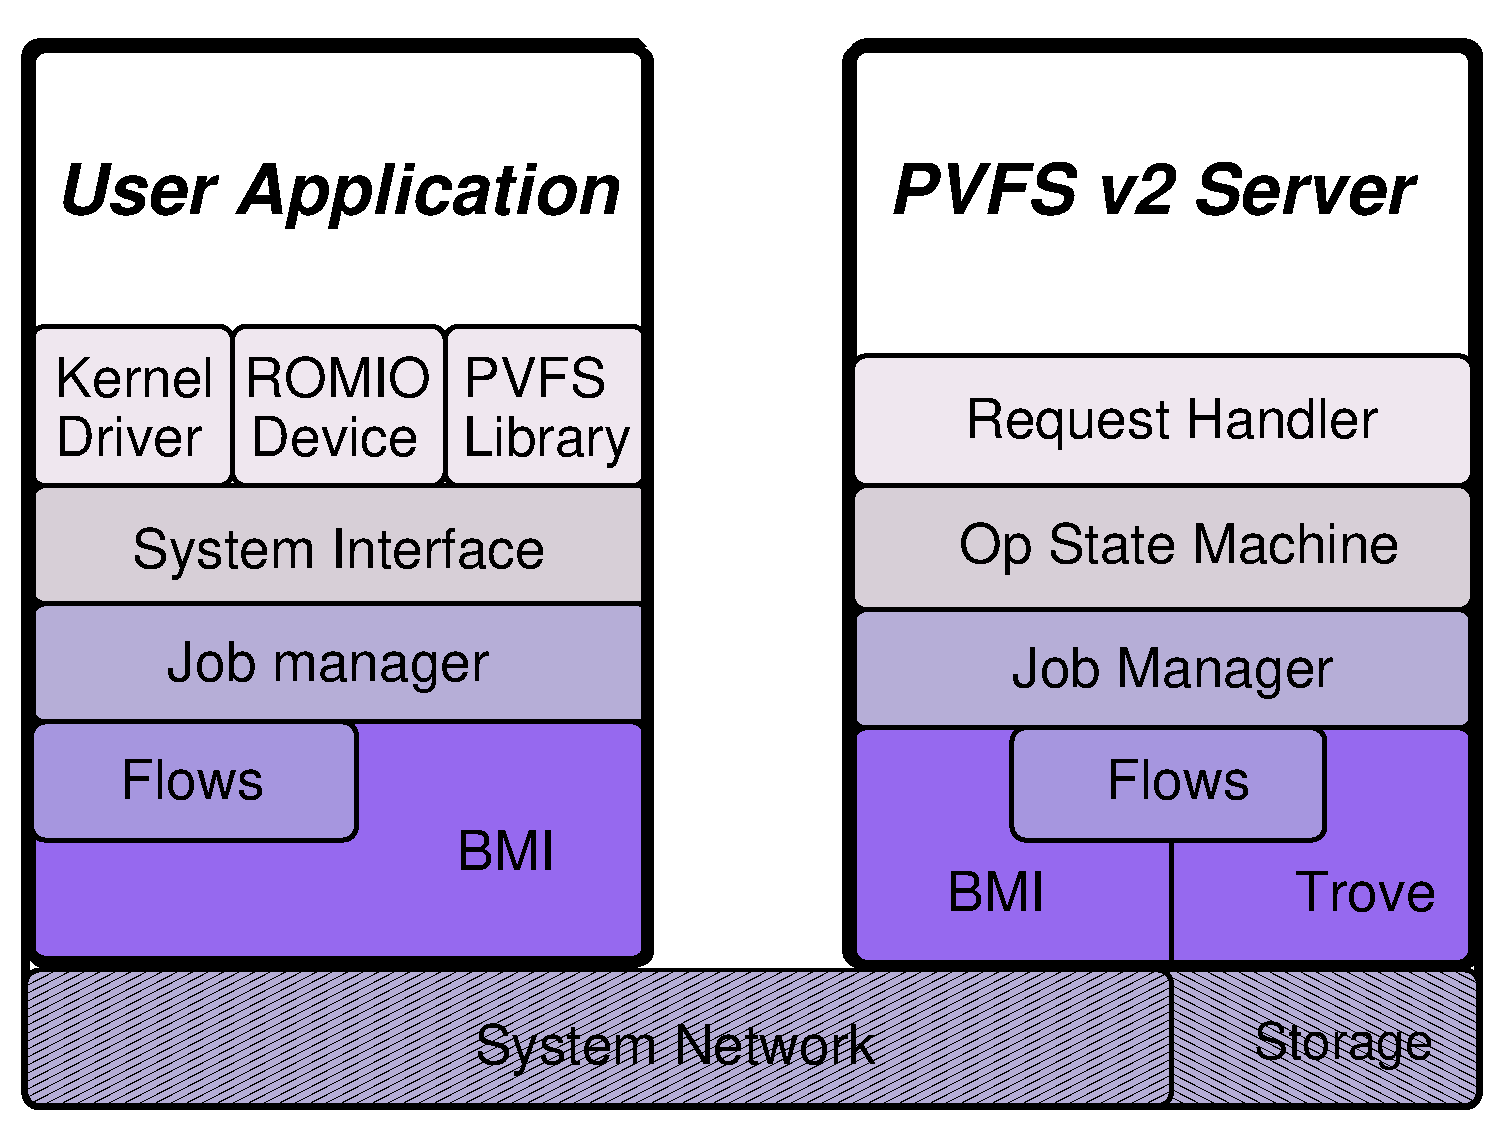
\includegraphics[scale=0.25]{interface-model.eps}
\caption{PVFS2 components \label{fig:interface-model}}
\end{figure}

\begin{figure}
\centering
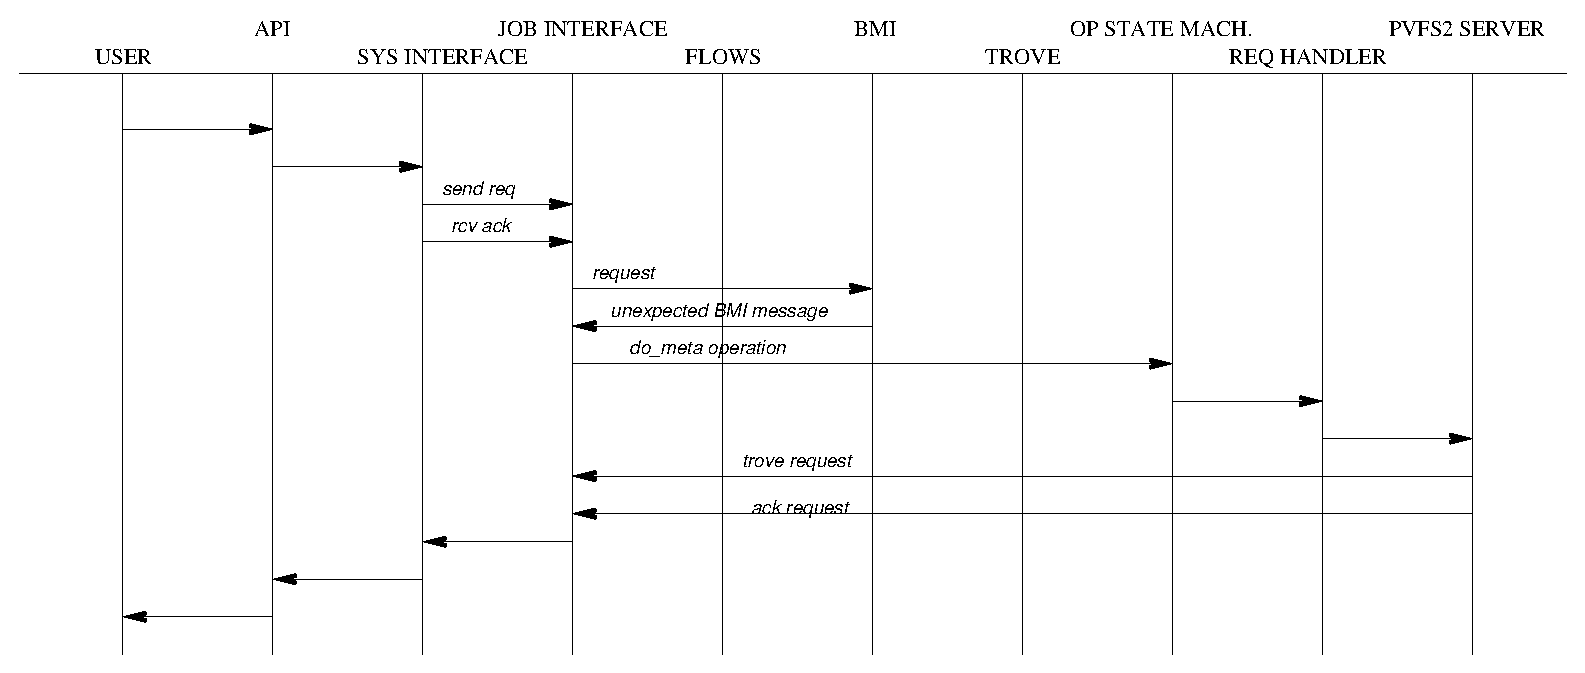
\includegraphics[scale=0.5]{setmeta-protocol.eps}
\caption{PVFS2 setmeta operation \label{fig:setmeta-protocol}}
\end{figure}

%\begin{figure}
%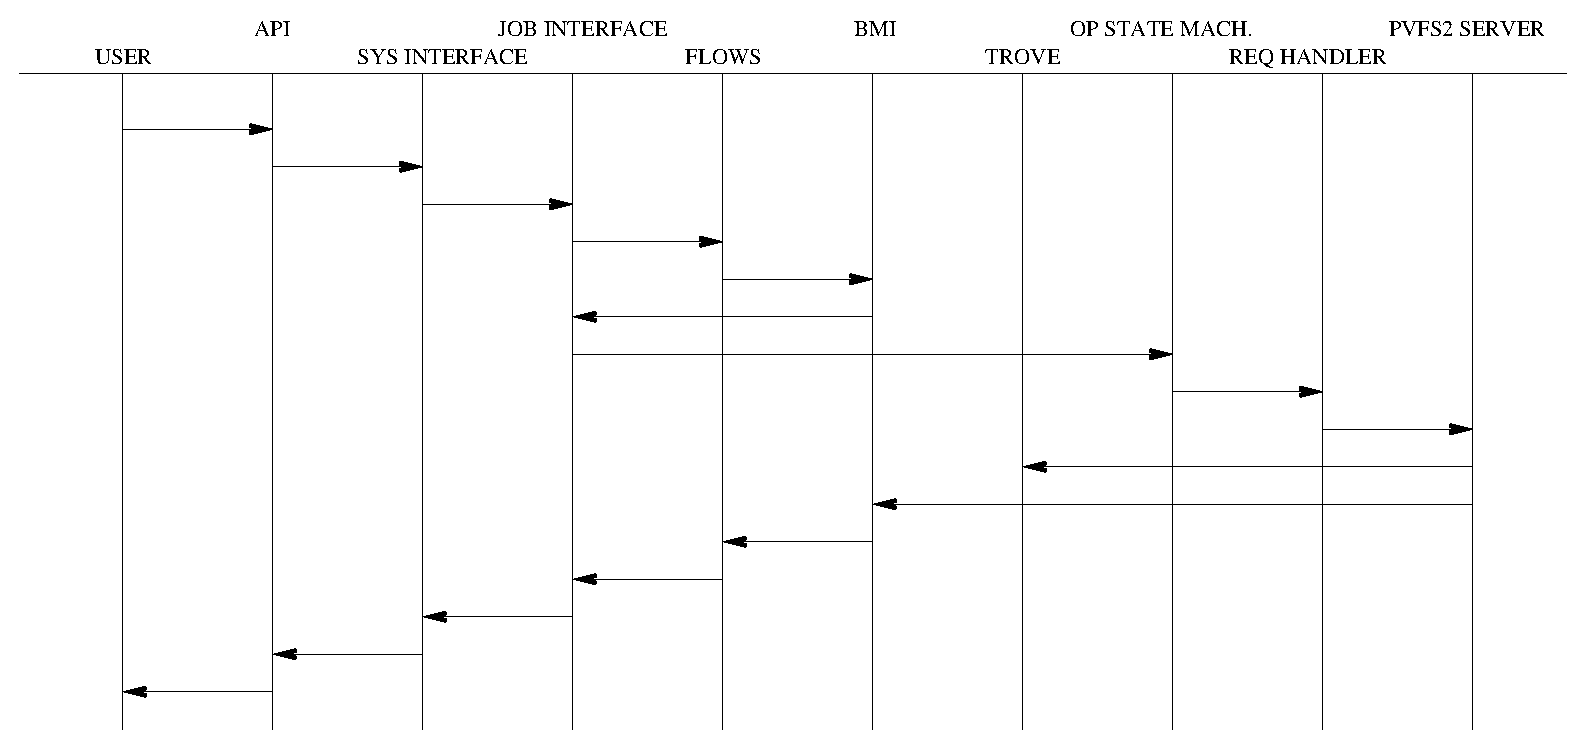
\includegraphics[scale=0.5]{io_op-protocol.eps}
%\caption{PVFS2 i/o (data) operation \label{fig:io-protocol}}
%\end{figure}

\end{document}
% vim: tw=72
